% \pdfminorversion=5
% \pdfcompresslevel=9
% \pdfobjcompresslevel=2
\documentclass[a4paper,12pt,reqno]{amsart}
\usepackage{M67tds}

% pour voir les solutions il faut enlever le commentaire de la ligne suivante
% \solutionstrue

\newlist{axioms}{description}{1}
\newcommand\axiomlabel[1]{\hfill\textbf{(#1)}}
\setlist[axioms]{style=nextline,before={\let\makelabel\axiomlabel}}
\newcommand*{\ensemble}[3][]{#1\{ #2 \;#1|\; #3 #1\}} % par exemple \ensemble[\big]{x^2}{x \in \R}
\newcommand*{\abs}[1]{\left\lvert{\ifx\hfuzz#1\hfuzz \,\cdot\,\else#1\fi}\right\rvert} % la valeur absolue
\newcommand*{\axiom}[1]{\textbf{(#1)}}
\newcommand*{\overeq}[1]{\overset{\tiny{#1}}{=}}

% Les notes de bas de page dans les minipages (sidebyside)
\renewcommand{\thempfootnote}{\fnsymbol{mpfootnote}}

% pour surligner
\sisolutions{
  \usepackage{soul}
  \colorlet{hl}{yellow!35!white}
  \sethlcolor{hl}
}

\begin{document}

% ==================================
\hautdepage{

\ifsolutions{Solutions de l'interrogation}\else{Interrogation}\fi\par\normalfont\normalsize
15 mars 2019\\{[ durée: 2 heures ]}\par
}
% ==================================
\sisujet{
  % {\fontencoding{U}\fontfamily{futs}\selectfont\char 66\relax}
  \tikz[baseline=(e.base)]{\NoAutoSpacing\node(e){!};\draw[red,ultra thick,line join=round,yshift=-.15ex](90:1em)--(210:1em)--(330:1em)--cycle;}
  \textbf{Documents autorisés :}\textit{Une feuille A4 recto-verso écrite à la main.}

  \vspace{17mm}
  \tsvp
}

%-----------------------------------
\begin{exo} (Construction à la règle et compas)

  Soient les deux points $O(0,0)$ et $I(1,0)$ du plan euclidien $\mathbb{R}^2$. Illustrer par un dessin et donner un programme de construction à la règle et au compas à partir de $O$ et $I$ :
  \begin{enumerate}
    \item des points $J(1,1)$ et $K(0,1)$\sisujet{\footnote{Il y avait une coquille dans le sujet imprimé, c'était $K(1,0)$.}} du carré $OIJK$;
    \item du point $L(1+\sqrt{2},-\frac{2}{3})$.
  \end{enumerate}
\end{exo}

\begin{solution}\def\C{\mathcal{C}}

  \begin{convention}
    On note $\C(X,Y)$ le cercle de centre $X$ passant par $Y$, $\C(X,YZ)$ le cercle de centre X et de rayon $YZ$ (qui est constructible si $X$, $Y$ et $Z$ le sont) et $\C^{*}(X,Y) = \C(X,Y)\setminus\{Y\}$.
  \end{convention}
  \sidebyside{.59}{
    \begin{enumerate}
      \item
      \begin{enumerate}[1.]
        \item $A(0,2)=\C^*(I,O) \cap (IO)$;
        \item $\{B_1,B_2\}=\C(O,A) \cap \C(A,O)$,\\ ainsi $(B_1B_2)$ est la médiatrice de $[OA]$;
        \item $\{J(1,1),J'(1,-1)\}=\C(I,O) \cap (B_1B_2)$;
        \item $K(0,1)=\C(O,I) \cap \C(J,I)$;
      \end{enumerate}
    \end{enumerate}
  }{
    \raisebox{-35mm}[0pt][0pt]{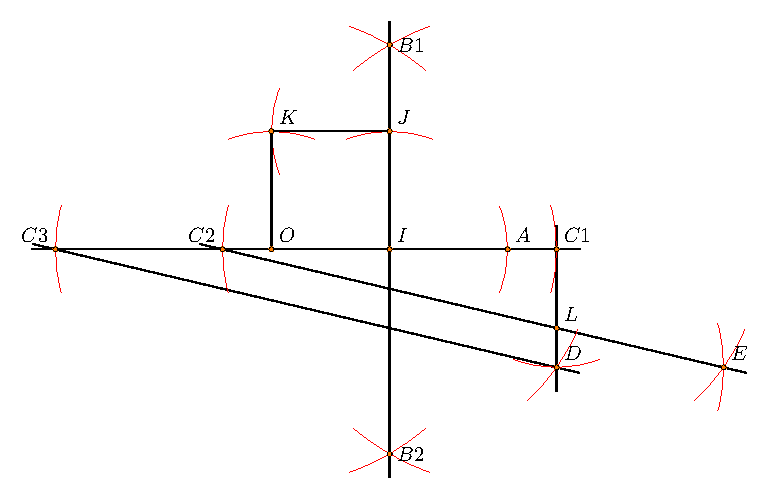
\includegraphics[width=7cm]{M67_2018-19_DS1_img_construction}}
  }
  \begin{enumerate}\setcounter{enumi}{1}
    \item
    \begin{enumerate}[1.]\setcounter{enumii}{4}
      \item $\{C_1(1+\sqrt{2},0),C_2(1-\sqrt{2},0)\}=\C(I,K) \cap (OI)$, car $IK=\sqrt{2}$;
      \item $C_3(1-2\sqrt{2},0)=\C^*(C_2,I) \cap (OI)$;
      \item $D(1+\sqrt{2},-1)=\C(C_1,JI) \cap \C(I,JC_1)$;
      \item $E=\C(D,C_3C_2) \cap \C(C_2,C_3D)$, de sorte que $(C_2E) // (C_3D)$;
      \item $L(1+\sqrt{2},-\frac{2}{3}) = (C_1D) \cap (C2E)$, car d'après Thalès $C_{1}L = C_{1}D \frac{C_1C_2}{C_1C_3} = 1 \frac{2\sqrt{2}}{3\sqrt{2}} = \frac{2}{3}$.
    \end{enumerate}
  \end{enumerate}
\end{solution}

\sisujet{\vspace{17mm}}

%-----------------------------------
\begin{exo} (Inégalité triangulaire, isométries)

  Soient $A,B,C$ trois points du plan euclidien $\mathbb{R}^{2}$.
  \begin{enumerate}
    \item Soient $A$, $B$ et $C$ alignés, montrer que $AC \leq AB+BC$, avec égalité si et seulement si $B \in [AC]$.
    \item Soient $A$, $B$ et $C$ non alignés, montrer que $AC < AB+BC$.
    \item En déduire que les isométries du plan euclidien préservent les alignements des points.
  \end{enumerate}
\end{exo}

\begin{solution}
  \begin{enumerate}
    \item\label{egtriang} Comme $A$, $B$ et $C$ sont alignés, il existe $\lambda \in \mathbb{R}$ tel que $B=(1- \lambda)A + \lambda C$. Donc $\vv{AB} = B - A = \lambda (C-A) = \lambda \vv{AC}$, ainsi $AB = \abs{\lambda} AC$. De même $\vv{CB} = B - C = (1-\lambda)(A-C) = (1-\lambda)\vv{CA}$, et donc $BC=\abs{1- \lambda}AC$. Ainsi $AB+BC = (\abs{\lambda}+\abs{1-\lambda})AC$, et comme $\abs{\lambda}+\abs{1-\lambda} \geq 1$ avec égalité si et seulement si $\lambda \in [0,1]$, on trouve que $AB+BC \geq AC$, avec égalité si et seulement si $B \in [AC]$.
    \item\label{inegtriang}\vspace{-2mm}
    \sidebyside{.7}{
      Soient $A$, $B$ et $C$ non alignés et $P$ la projection orthogonale de $B$ sur $(AC)$. Comme $BP>0$, nous avons d'après Pythagore $AB > AP$ et $BC > PC$. Ainsi $AB+BC > AP+PC \geq AC$.
    }{
      \raisebox{-14mm}[0pt][0pt]{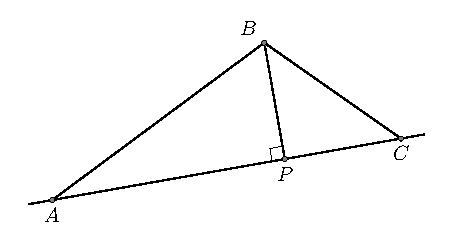
\includegraphics[width=4cm]{M67_2018-19_DS1_img_inegtraing}}
    }\vspace{3mm}
    \item Soient $f$ une isométrie et $A$, $B$, $C$ trois points alignés dans cet ordre, avec $B \in [AC]$. Nous avons $f(A)f(B) + f(B)f(C) = AB + BC$ et $AC = f(A)f(C)$, car $f$ est une isométrie, et $AB + BC = AC$ d'après \ref{egtriang}). Ainsi $f(A)f(B) + f(B)f(C) = f(A)f(C)$ et donc, d'après \ref{inegtriang}), les points $f(A)$, $f(B)$, $f(C)$ sont alignés\footnote{dans cet ordre, d'après \ref{egtriang})}, en particulier $f$ préserve l'alignement des points.
  \end{enumerate}
\end{solution}

\sisujet{\newpage}

%-----------------------------------
\begin{exo} (Axiomatique)

  On rappelle les propriétés d'incidence et d'ordre:\\[-1.7\baselineskip]
  \begin{multicols}{2}\small
    \begin{axioms}[leftmargin=3.5em]
      \item[I1] par deux points distincts passe une unique droite,
      \item[I2] toute droite contient au moins deux points distincts,
      \item[I3] il existe trois points non alignés,
      \item[O1] si $C$ est entre $A$ et $B$, $B$ et $C$ sont alignés, deux à deux distincts et $C$ est aussi entre $B$ et $A$,
      \item[O2] pour tous points distincts $A$ et $B$ il existe un point $C$ tel que $B$ soit entre $A$ et $C$,
      \item[O3] parmi trois points alignés deux à deux distincts, un et un seul d'entre eux est entre les deux autres,
      \item[O4] soient $A$, $B$, et $C$ trois points non alignés et $\ens{D}$ une droite ne passant par aucun d'eux. Si $\ens{D}$ passe par un point $D$ entre $A$ et $B$, alors $\ens{D}$ passe ou bien par un point entre $A$ et $C$, ou bien par un point entre $B$ et $C$, mais pas les deux à la fois.
    \end{axioms}
  \end{multicols}\vspace{7pt}
    Soient $A$, $B$ et $C$ trois points non alignés, $I$ un point entre $B$ et $C$, $J$ un point entre $A$ et $C$.
    \begin{enumerate}
      \item Montrer que la droite $(AI)$ est distincte des droites $(AB)$ et $(AC)$.
      \item Montrer que $(AI)$ passe par un point $O$ entre $B$ et $J$.
      \item Montrer que $O$ est entre $A$ et $I$.
      \item Montrer que $(CO)$ passe par un point $K$ entre $A$ et $B$, puis que $O$ est entre $C$ et $K$.
    \end{enumerate}
    \sisujet{\emph{On dit que le point $O$ est à l'intérieur du triangle $\tri ABC$.}}
\end{exo}

\begin{solution}

  Comme $A$, $B$ et $C$ sont non alignés, les droites $(AB)$, $(BC)$ et $(CA)$ sont bien définies. De plus comme $I$ est aligné avec $B$ et $C$, d'après \axiom{O1}, alors $I \neq A$ et donc la droite $(AI)$ est bien définie. De même, les droites $(BJ)$ et $(CK)$ sont bien définies.
  \begin{enumerate}
    \item\label{nonalign}%\vspace{-2mm}
    \sidebyside{.7}{
      Supposons que $(AI) = (AB)$, alors $(AB) \overeq{\axiom{I1}+\axiom{O1}} (BI) \overeq{\axiom{O1}}  (BC)$, ce qui est en contradiction avec le fait que $A$, $B$ et $C$ sont non alignés, donc $(AI) \neq (AB)$. De même $(AI) \neq (AC)$.
    }{
      \hfill\raisebox{-17mm}[0pt][0pt]{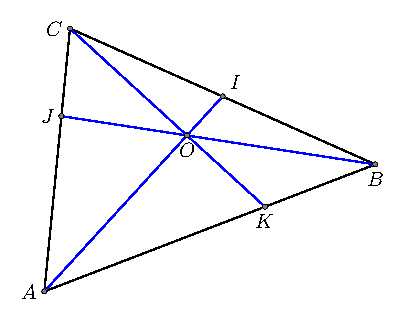
\includegraphics[width=4cm]{M67_2018-19_DS1_img_point_interieur}}
    }\vspace{3mm}
    \item Remarquons d'abord que la droite $(AI)$ ne passe par aucun des trois points $J$,$C$ et $B$ car sinon on aurait $(AI) = (AC)$ ou $(AI) = (AB)$ en contradiction avec la question précédente. Donc on peut appliquer $\axiom{O4}$ à la droite $(AI)$ et les points $B$,$J$ et $C$. La droite $(AI)$ ne passe pas entre $J$ et $C$, car sinon $(AC) = (AI)$ vu qu'on aurait en plus de $A$ un autre\footnote{car $A$ n'est pas entre $J$ et $C$ d'après \axiom{O3}.} point qui serait sur ces deux droites. Ainsi on trouve que $(AI)$ passe par un point $O$ entre $B$ et $J$.
    \item\label{entreentre} D'après la question précédente, appliquée à $J$ à la place de $I$, on trouve que $(BJ)$ passe par un point $O'$ entre $A$ et $I$. Si on suppose que $O \neq O'$, on aurait ces deux points sur les droites $(AI)$ et $(BJ)$, qui doivent ainsi coïncider, et donc $(AI) = (AJ)\overeq{\axiom{O1}}(AC)$ serait en contradiction avec \ref{nonalign}). Ainsi $O=O'$ est entre $A$ et $I$.
    \item D'après \ref{nonalign}) appliqué aux points $C$, $A$, $I$ et $O$ nous avons $(CO)\neq(CI)\overeq{\axiom{O1}}(CB)$ et $(CO)\neq(CA)$, ainsi $(CO)$ ne passe par aucun des points $A$, $B$ et $I$, ni par un point entre $B$ et $I$. Donc on peut appliquer \axiom{O4} à la droite $(CO)$ et les points $A$,$B$ et $I$ pour conclure que $(CO)$ passe par un point $K$ entre $A$ et $B$. Pour conclure que $O$ est entre $C$ et $K$ il suffit d'appliquer la question \ref{entreentre}) avec $C$ et $K$ à la place de $A$ et $I$.
  \end{enumerate}
\end{solution}


\end{document}
